\documentclass[tikz]{standalone}
\usepackage{tikz,amsmath}
\usetikzlibrary{calc}
\begin{document}
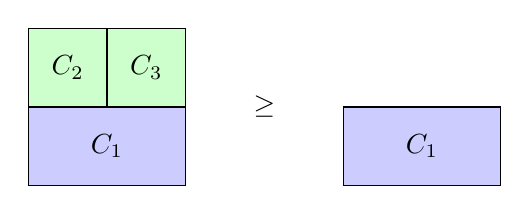
\begin{tikzpicture}
    \draw [fill=green!20] (0,0) -- (0,2) -- (2,2) -- (2,0) --cycle;
    \draw [fill=blue!20] (0,0) -- (0,1) -- (2,1) -- (2,0) --cycle;
    \draw (1,1) -- (1,2);
    \node at (1,.5) {$C_1$};
    \node at (.5,1.5) {$C_2$};
    \node at (1.5,1.5) {$C_3$};
    \node at (3,1) {$\geq$};
    \draw [fill=blue!20,xshift=4cm] (0,0) -- (0,1) -- (2,1) -- (2,0) --cycle;
    \node [xshift=4cm] at (1,.5) {$C_1$};
\end{tikzpicture}
\end{document}
